\section{Developer zone: In memory representation}
Network modelling can be mathematically abstracted into a graph of stations (graph nodes) and pipes or active network elements (graph edges). The network graph is implemented using Boost Graph Library, which provides a labeled graph implementation and related algorithms. The network data in particular is stored into the graph labels. Shimmer++ represents the network as an undirected graph, therefore pipes are inherently not directional, in contrast to physical variables as velocity or flux. Using the facilities of the Boost Graph Library, the definition of the graph type is
\begin{verbatim}
    using infrastructure_graph = adjacency_list< listS, vecS,
                                    undirectedS, vertex_properties, edge_properties>;    
\end{verbatim}    
which is found in \texttt{shimmer++/src/infrastructure\_graph.h}. In turn, the graph
labels have the following types:
\begin{minted}[linenos=true,numbersep=1pt,frame=lines,framesep=0.5mm]{cpp}
 using namespace boost;

 using infrastructure_graph = adjacency_list< listS, vecS,
                                    undirectedS, vertex_properties, edge_properties>;
 using sptr_pipe_t = std::shared_ptr<edge_station::station>; 
 using uptr_node_t = std::unique_ptr<station>;
 
 struct vertex_properties                       
 {                                              
    int             u_snum;                     
    int             i_snum;                     
    station_type    type;                       
    double          height;                     
    double          latitude;                   
    double          longitude;                  
    vector_t        gas_mixture;                
    uptr_node_t     node_station;               
                                                  
 };

 struct edge_properties 
 {
    pipe_type   type;
    int         branch_num;
    double      length;
    double      diameter;
    double      friction_factor;
    sptr_pipe_t pipe_station;
    std::string name;
    int         i_sfrom;
    int         i_sto;          
 };  

 enum class pipe_type = { pipe, resistor, compressor, regulator,  valve};
\end{minted}

    
%\begin{tikzpicture}[remember picture,overlay]
%    \def\a{-0.5}
%    \draw[dpipe] ( 8.0, 2+\a) -- ( 8.0, 7.00) -- (14.5, 7.00) -- (14.5, 2+\a) -- cycle;
%    \draw[dnode] (-0.5, 2+\a) -- (-0.5, 7.00) -- ( 6  , 7.00) -- ( 6 , 2+\a) -- cycle;
%\end{tikzpicture}

Network graphs are populated via network data files by the user however, from the developer point of view, it could be useful to populate them manually. For the first option see Section \ref{SectionDatabase}. In the second case, you will need to introduce pipe and node properties one by one as will explained in what follows. Lets take as example the graph in Fig. \ref{fig: graph_example} of a simplified  gas network. 

\begin{figure}[H]
    \centering
            % Graphic for TeX using PGF
% Title: /home/karol/Documents/UNIVERSITA/POLITO/PRESENTATIONS/SHIMMER_2024_01/img_code/pipe_network.dia
% Creator: Dia v0.97.3
% CreationDate: Mon Jan 22 14:43:56 2024
% For: karol
% \usepackage{tikz}
% The following commands are not supported in PSTricks at present
% We define them conditionally, so when they are implemented,
% this pgf file will use them.
\ifx\du\undefined
  \newlength{\du}
\fi
\setlength{\du}{11\unitlength}
\begin{tikzpicture}[even odd rule]
\pgftransformxscale{1.000000}
\pgftransformyscale{-1.000000}
\definecolor{dialinecolor}{rgb}{0.000000, 0.000000, 0.000000}
\pgfsetstrokecolor{dnode}
\pgfsetstrokeopacity{1.000000}
\definecolor{diafillcolor}{rgb}{1.000000, 1.000000, 1.000000}
\pgfsetfillcolor{diafillcolor}
\pgfsetfillopacity{1.000000}
\pgfsetlinewidth{0.100000\du}
\pgfsetdash{}{0pt}
\pgfsetmiterjoin
\definecolor{diafillcolor}{rgb}{1.000000, 1.000000, 1.000000}
\pgfsetfillcolor{diafillcolor}
\pgfsetfillopacity{1.000000}
\pgfpathellipse{\pgfpoint{8.693572\du}{5.676288\du}}{\pgfpoint{0.693572\du}{0\du}}{\pgfpoint{0\du}{0.676288\du}}
\pgfusepath{fill}
\definecolor{dialinecolor}{rgb}{0.937255, 0.000000, 0.701961}
\pgfsetstrokecolor{dnode}
\pgfsetstrokeopacity{1.000000}
\pgfpathellipse{\pgfpoint{8.693572\du}{5.676288\du}}{\pgfpoint{0.693572\du}{0\du}}{\pgfpoint{0\du}{0.676288\du}}
\pgfusepath{stroke}
% setfont left to latex
% setfont left to latex
\definecolor{dialinecolor}{rgb}{0.000000, 0.000000, 0.000000}
\pgfsetstrokecolor{dnode}
\pgfsetstrokeopacity{1.000000}
\definecolor{diafillcolor}{rgb}{0.000000, 0.000000, 0.000000}
\pgfsetfillcolor{diafillcolor}
\pgfsetfillopacity{1.000000}
\node[anchor=base,inner sep=0pt, outer sep=0pt,color=dnode] at (8.693572\du,5.961288\du){0};
\pgfsetlinewidth{0.100000\du}
\pgfsetdash{}{0pt}
\pgfsetmiterjoin
\definecolor{diafillcolor}{rgb}{1.000000, 1.000000, 1.000000}
\pgfsetfillcolor{diafillcolor}
\pgfsetfillopacity{1.000000}
\pgfpathellipse{\pgfpoint{8.693572\du}{9.676288\du}}{\pgfpoint{0.693572\du}{0\du}}{\pgfpoint{0\du}{0.676288\du}}
\pgfusepath{fill}
\definecolor{dialinecolor}{rgb}{0.937255, 0.000000, 0.701961}
\pgfsetstrokecolor{dnode}
\pgfsetstrokeopacity{1.000000}
\pgfpathellipse{\pgfpoint{8.693572\du}{9.676288\du}}{\pgfpoint{0.693572\du}{0\du}}{\pgfpoint{0\du}{0.676288\du}}
\pgfusepath{stroke}
% setfont left to latex
% setfont left to latex
\definecolor{dialinecolor}{rgb}{0.000000, 0.000000, 0.000000}
\pgfsetstrokecolor{dialinecolor}
\pgfsetstrokeopacity{1.000000}
\definecolor{diafillcolor}{rgb}{0.000000, 0.000000, 0.000000}
\pgfsetfillcolor{diafillcolor}
\pgfsetfillopacity{1.000000}
\node[anchor=base,inner sep=0pt, outer sep=0pt,color=dnode] at (8.693572\du,9.961288\du){1};
\pgfsetlinewidth{0.100000\du}
\pgfsetdash{}{0pt}
\pgfsetmiterjoin
\definecolor{diafillcolor}{rgb}{1.000000, 1.000000, 1.000000}
\pgfsetfillcolor{diafillcolor}
\pgfsetfillopacity{1.000000}
\pgfpathellipse{\pgfpoint{6.753572\du}{13.676288\du}}{\pgfpoint{0.753572\du}{0\du}}{\pgfpoint{0\du}{0.676288\du}}
\pgfusepath{fill}
\definecolor{dialinecolor}{rgb}{0.937255, 0.000000, 0.701961}
\pgfsetstrokecolor{dnode}
\pgfsetstrokeopacity{1.000000}
\pgfpathellipse{\pgfpoint{6.753572\du}{13.676288\du}}{\pgfpoint{0.753572\du}{0\du}}{\pgfpoint{0\du}{0.676288\du}}
\pgfusepath{stroke}
% setfont left to latex
% setfont left to latex
\definecolor{dialinecolor}{rgb}{0.000000, 0.000000, 0.000000}
\pgfsetstrokecolor{dialinecolor}
\pgfsetstrokeopacity{1.000000}
\definecolor{diafillcolor}{rgb}{0.000000, 0.000000, 0.000000}
\pgfsetfillcolor{diafillcolor}
\pgfsetfillopacity{1.000000}
\node[anchor=base,inner sep=0pt, outer sep=0pt,color=dnode] at (6.753572\du,13.961288\du){2};
\pgfsetlinewidth{0.100000\du}
\pgfsetdash{}{0pt}
\pgfsetmiterjoin
\definecolor{diafillcolor}{rgb}{1.000000, 1.000000, 1.000000}
\pgfsetfillcolor{diafillcolor}
\pgfsetfillopacity{1.000000}
\pgfpathellipse{\pgfpoint{14.693572\du}{13.676288\du}}{\pgfpoint{0.693572\du}{0\du}}{\pgfpoint{0\du}{0.676288\du}}
\pgfusepath{fill}
\definecolor{dialinecolor}{rgb}{0.937255, 0.000000, 0.701961}
\pgfsetstrokecolor{dnode}
\pgfsetstrokeopacity{1.000000}
\pgfpathellipse{\pgfpoint{14.693572\du}{13.676288\du}}{\pgfpoint{0.693572\du}{0\du}}{\pgfpoint{0\du}{0.676288\du}}
\pgfusepath{stroke}
% setfont left to latex
% setfont left to latex
\definecolor{dialinecolor}{rgb}{0.000000, 0.000000, 0.000000}
\pgfsetstrokecolor{dialinecolor}
\pgfsetstrokeopacity{1.000000}
\definecolor{diafillcolor}{rgb}{0.000000, 0.000000, 0.000000}
\pgfsetfillcolor{diafillcolor}
\pgfsetfillopacity{1.000000}
\node[anchor=base,inner sep=0pt, outer sep=0pt,color=dnode] at (14.693572\du,13.961288\du){4};
\pgfsetlinewidth{0.100000\du}
\pgfsetdash{}{0pt}
\pgfsetmiterjoin
\definecolor{diafillcolor}{rgb}{1.000000, 1.000000, 1.000000}
\pgfsetfillcolor{diafillcolor}
\pgfsetfillopacity{1.000000}
\pgfpathellipse{\pgfpoint{10.693572\du}{13.676288\du}}{\pgfpoint{0.693572\du}{0\du}}{\pgfpoint{0\du}{0.676288\du}}
\pgfusepath{fill}
\definecolor{dialinecolor}{rgb}{0.937255, 0.000000, 0.701961}
\pgfsetstrokecolor{dnode}
\pgfsetstrokeopacity{1.000000}
\pgfpathellipse{\pgfpoint{10.693572\du}{13.676288\du}}{\pgfpoint{0.693572\du}{0\du}}{\pgfpoint{0\du}{0.676288\du}}
\pgfusepath{stroke}
% setfont left to latex
% setfont left to latex
\definecolor{dialinecolor}{rgb}{0.000000, 0.000000, 0.000000}
\pgfsetstrokecolor{dialinecolor}
\pgfsetstrokeopacity{1.000000}
\definecolor{diafillcolor}{rgb}{0.000000, 0.000000, 0.000000}
\pgfsetfillcolor{diafillcolor}
\pgfsetfillopacity{1.000000}
\node[anchor=base,inner sep=0pt, outer sep=0pt,color=dnode] at (10.693572\du,13.961288\du){3};
\pgfsetlinewidth{0.050000\du}
\pgfsetdash{}{0pt}
\pgfsetbuttcap
{
\definecolor{diafillcolor}{rgb}{0.000000, 0.501961, 0.501961}
\pgfsetfillcolor{diafillcolor}
\pgfsetfillopacity{1.000000}
% was here!!!
\definecolor{dialinecolor}{rgb}{0.000000, 0.501961, 0.501961}
\pgfsetstrokecolor{dpipe}
\pgfsetstrokeopacity{1.000000}
\draw (8.693572\du,6.351417\du)--(8.693570\du,9.000000\du);
}
\pgfsetlinewidth{0.050000\du}
\pgfsetdash{}{0pt}
\pgfsetbuttcap
{
\definecolor{diafillcolor}{rgb}{0.000000, 0.501961, 0.501961}
\pgfsetfillcolor{diafillcolor}
\pgfsetfillopacity{1.000000}
% was here!!!
\definecolor{dialinecolor}{rgb}{0.000000, 0.501961, 0.501961}
\pgfsetstrokecolor{dpipe}
\pgfsetstrokeopacity{1.000000}
\draw (8.693570\du,10.352600\du)--(6.753570\du,13.000000\du);
}
\pgfsetlinewidth{0.050000\du}
\pgfsetdash{}{0pt}
\pgfsetbuttcap
{
\definecolor{diafillcolor}{rgb}{0.000000, 0.501961, 0.501961}
\pgfsetfillcolor{diafillcolor}
\pgfsetfillopacity{1.000000}
% was here!!!
\definecolor{dialinecolor}{rgb}{0.000000, 0.501961, 0.501961}
\pgfsetstrokecolor{dpipe}
\pgfsetstrokeopacity{1.000000}
\draw (8.693570\du,10.352600\du)--(10.693600\du,13.000000\du);
}
\pgfsetlinewidth{0.050000\du}
\pgfsetdash{}{0pt}
\pgfsetbuttcap
{
\definecolor{diafillcolor}{rgb}{0.000000, 0.501961, 0.501961}
\pgfsetfillcolor{diafillcolor}
\pgfsetfillopacity{1.000000}
% was here!!!
\definecolor{dialinecolor}{rgb}{0.000000, 0.501961, 0.501961}
\pgfsetstrokecolor{dpipe}
\pgfsetstrokeopacity{1.000000}
\draw (10.000000\du,13.676300\du)--(7.507140\du,13.676300\du);
}
\pgfsetlinewidth{0.050000\du}
\pgfsetdash{}{0pt}
\pgfsetbuttcap
{
\definecolor{diafillcolor}{rgb}{0.000000, 0.501961, 0.501961}
\pgfsetfillcolor{diafillcolor}
\pgfsetfillopacity{1.000000}
% was here!!!
\definecolor{dialinecolor}{rgb}{0.000000, 0.501961, 0.501961}
\pgfsetstrokecolor{dpipe}
\pgfsetstrokeopacity{1.000000}
\draw (11.387100\du,13.676300\du)--(14.000000\du,13.676300\du);
}
% setfont left to latex
% setfont left to latex
\definecolor{dialinecolor}{rgb}{0.000000, 0.501961, 0.501961}
\pgfsetstrokecolor{dialinecolor}
\pgfsetstrokeopacity{1.000000}
\definecolor{diafillcolor}{rgb}{0.000000, 0.501961, 0.501961}
\pgfsetfillcolor{diafillcolor}
\pgfsetfillopacity{1.000000}
\node[anchor=base west,inner sep=0pt,outer sep=0pt,color=dpipe] at (7.5000000\du,8.000000\du){0};
% setfont left to latex
% setfont left to latex
\definecolor{dialinecolor}{rgb}{0.000000, 0.501961, 0.501961}
\pgfsetstrokecolor{dialinecolor}
\pgfsetstrokeopacity{1.000000}
\definecolor{diafillcolor}{rgb}{0.000000, 0.501961, 0.501961}
\pgfsetfillcolor{diafillcolor}
\pgfsetfillopacity{1.000000}
\node[anchor=base west,inner sep=0pt,outer sep=0pt,color=dpipe] at (6.5000000\du,12.000000\du){3};
% setfont left to latex
% setfont left to latex
\definecolor{dialinecolor}{rgb}{0.000000, 0.501961, 0.501961}
\pgfsetstrokecolor{dialinecolor}
\pgfsetstrokeopacity{1.000000}
\definecolor{diafillcolor}{rgb}{0.000000, 0.501961, 0.501961}
\pgfsetfillcolor{diafillcolor}
\pgfsetfillopacity{1.000000}
\node[anchor=base west,inner sep=0pt,outer sep=0pt,color=dpipe] at (10.5000000\du,12.000000\du){1};
% setfont left to latex
% setfont left to latex
\definecolor{dialinecolor}{rgb}{0.000000, 0.501961, 0.501961}
\pgfsetstrokecolor{dialinecolor}
\pgfsetstrokeopacity{1.000000}
\definecolor{diafillcolor}{rgb}{0.000000, 0.501961, 0.501961}
\pgfsetfillcolor{diafillcolor}
\pgfsetfillopacity{1.000000}
\node[anchor=base west,inner sep=0pt,outer sep=0pt,color=dpipe] at (8.450000\du,14.900000\du){2};
% setfont left to latex
% setfont left to latex
\definecolor{dialinecolor}{rgb}{0.000000, 0.501961, 0.501961}
\pgfsetstrokecolor{dialinecolor}
\pgfsetstrokeopacity{1.000000}
\definecolor{diafillcolor}{rgb}{0.000000, 0.501961, 0.501961}
\pgfsetfillcolor{diafillcolor}
\pgfsetfillopacity{1.000000}
\node[anchor=base west,inner sep=0pt,outer sep=0pt,color=dpipe] at (12.590000\du,14.895000\du){4};
\end{tikzpicture}
    
    \caption{Graph representation of a simplified gas network.}
    \label{fig: graph_example}
\end{figure}

\subsection{Define the graph}
In the main function add the definition of the graph. For the sake of clearness, let us proceed step by step and introduce two functions aimed to add first the vertex, \texttt{make\_init\_vertex} and later on the pipes properties, \texttt{make\_init\_pipes}. 

\begin{minted}[linenos=true,numbersep=5pt,frame=lines,framesep=0.5mm ]{cpp}
    int main()
    {
        infrastructure_graph igraph;
        std::vector<vertex_descriptor> vds;
        make_init_vertex(igraph, vds);
        make_init_pipes(igraph, vds);
    
        return 0; 
    }
\end{minted}   


\subsection{Add nodes specification}
Let us suppose that the data shown in Tab. \ref{tab: node_data} is attached to the network vertices. For this example, no specification about mixture composition is  taken into account. Nonetheless, this functionality is supported and can be easily added.

\begin{table}[H]
    \centering
       \begin{tabular}{ccrrrcccc}
        & & & & & & & & \\
        \hline 
        &  & \multicolumn{3}{c}{Node properties}  & & \multicolumn{3}{c}{Mixture composition} \\ \cline{3-5} \cline{7-9}     
        \multirow{5}{*}{\rotatebox[origin=c]{90}{\cnodes{Nodes}}} 
        &           & G[kg/s] &p[Pa] &H[m]  && CH4 & N2& {\dots} \\ \hline
        &\cnodes{0} &	\cellcolor{dnode!30} 5000  & \cellcolor{dnode!30}-60  &\cellcolor{dnode!30}10.0  && -& -& -\\
        &\cnodes{1} &\cellcolor{dnode!30}	0	  &\cellcolor{dnode!30}  20  &\cellcolor{dnode!30} 20.0  && -& - & {-}\\
        &\cnodes{2} &\cellcolor{dnode!30}	0	  & \cellcolor{dnode!30} 25  &\cellcolor{dnode!30} 30.0  && -& - & {-}\\ 
        &\cnodes{3} &\cellcolor{dnode!30}	0	  &\cellcolor{dnode!30}  35  &\cellcolor{dnode!30}40.0  && -& - &  {-}\\ 
        &\cnodes{4} &\cellcolor{dnode!30}	0	  &\cellcolor{dnode!30}  50  &\cellcolor{dnode!30}50.0  && -& - & {-}\\
        \hline
        &&&&&&&&\\
        \end{tabular}
    \caption{Parameters concerning node specification.}
    \label{tab: node_data}
\end{table}
 
%\begin{tikzpicture}[remember picture,overlay]
%    \draw[dnode] (9.3, 1.3) -- (9.3,2.85) -- ( 7.15, 2.85) -- (7.15, 1.3) -- cycle;
%\end{tikzpicture}

        
%\begin{tikzpicture}[remember picture,overlay]
%    \draw[dpipe](10.2, 0.8) -- (10.2, 3.10) -- (13.5, 3.10) -- (13.5, 0.8) -- cycle;
%    \draw[dnode]( 2.0, 0.8) -- (2.0, 3.10) -- ( 4.7, 3.10) -- ( 4.7, 0.8) -- cycle;
%\end{tikzpicture}

%In the following snippet code you will distinguish a lambda function called \texttt{add\_vertex}, which internally call the \texttt{boost::add\_vertex}. For the sake of simplicity, this will not be further explained, but keep in mind this is needed for the management of internal pointers in the vertex properties. 
%The vector \texttt{vds} stores the nodes created, which will be used in the following for the definition of the edges.

In the following snippet code, you will distinguish a std::vector \texttt{vds} and a lambda function called \texttt{add\_vertex} (see line 6), which internally calls the \texttt{boost::add\_vertex}. The first one is used for the storage of all nodes created at the \texttt{add\_vertex} call  and it will be used in the following for the definition of the edges. For the sake of simplicity, the lambda \texttt{add\_vertex} will not be further explained, but keep in mind it  is needed for the management of internal pointers in the vertex properties, associated to its non-pipe elements. 

\begin{minted}[linenos=true,numbersep=1pt,frame=lines,framesep=2mm]{cpp}
static void
make_init_vertex(infrastructure_graph& igraph, std::vector<vertex_descriptor>& vds)
{
    auto add_vertex = [&](vertex_properties&& vp) 
    {
        auto v = boost::add_vertex(igraph);
        igraph[v] = std::move(vp);
        return v;
    };

    // Insert station config (name, no., pressure, flux, height)
    vds.push_back( add_vertex( vertex_properties( "station 0", 0, 5000.,-60, 10. )) );
    vds.push_back( add_vertex( vertex_properties( "station 1", 1,    0., 20, 20. )) );
    vds.push_back( add_vertex( vertex_properties( "station 2", 2,    0., 25, 30. )) );
    vds.push_back( add_vertex( vertex_properties( "station 3", 3,    0., 35, 40. )) );
    vds.push_back( add_vertex( vertex_properties( "station 4", 4,    0., 50, 50. )) );
}
\end{minted}

\subsection{Add pipes specification}
Let us now continue with the \cpipes{pipes} specification using the values in Tab. \ref{tab: pipe_specification}. 


\begin{table}[H]
    \centering
            \begin{tabular}{cccccrrr}
            & & & & & & & \\
            \hline
            &  & \multicolumn{2}{c}{Nodes}&&\multicolumn{3}{c}{Pipe properties} \\ \cline{3-4} \cline{6-8}    
            &  & In	&Out	&&L[m]	&D[m]	&epsi[m] \\ \hline
            \multirow{5}{*}{\rotatebox[origin=c]{90}{\cpipes{Pipes}}}
            & \cpipes{0} &	\cnodes{0} &	\cnodes{1} &&	{\cellcolor{dpipe!30}} 80.0  &{\cellcolor{dpipe!30}}0.6	&{\cellcolor{dpipe!30}}1.2e-5 \\
            &\cpipes{1} &	\cnodes{1} &	\cnodes{3} &&{\cellcolor{dpipe!30}}	90.0  &{\cellcolor{dpipe!30}}0.5	&{\cellcolor{dpipe!30}}1.3e-5 \\
            &\cpipes{2} &	\cnodes{3} &	\cnodes{2} &&{\cellcolor{dpipe!30}}	100.0 &{\cellcolor{dpipe!30}}0.4	&{\cellcolor{dpipe!30}}1.4e-5 \\ 
            &\cpipes{3} &	\cnodes{1} &	\cnodes{2} &&{\cellcolor{dpipe!30}}	110.0 &{\cellcolor{dpipe!30}}0.3	&{\cellcolor{dpipe!30}}1.5e-5 \\ 
            &\cpipes{4} &	\cnodes{3} &	\cnodes{4} &&{\cellcolor{dpipe!30}}	120.0 &{\cellcolor{dpipe!30}}0.2	&{\cellcolor{dpipe!30}}1.6e-5 \\ \hline 
            &&&&&&& \\
            \end{tabular}
    \caption{Parameters concerning pipe specification.}
    \label{tab: pipe_specification}
\end{table}
In order to add the properties, first create an object of type \texttt{edge\_properties} instantiating it with the data related to the pipes: length, diameter and factor epsi.   Afterwards, the edges of the graph are created using the \texttt{boost::add\_edges} function while insertions of the pipes properties are given as parameters. The first two entrances (arguments) are the nodes defining the edge (two first columns in Tab. \ref{tab: pipe_specification}) followed by the object with  its corresponding properties. 

\begin{minted}[linenos=true,numbersep=1pt,frame=lines,framesep=2mm]{cpp}
static void
make_init_pipes(infrastructure_graph& igraph, std::vector<vertex_descriptor>& vds)
{
    edge_properties ep0  = {pipe_type::pipe, 0,   80, 0.6, 1.2e-5};
    edge_properties ep1  = {pipe_type::pipe, 1,   90, 0.5, 1.3e-5};
    edge_properties ep2  = {pipe_type::pipe, 2,  100, 0.4, 1.4e-5};
    edge_properties ep3  = {pipe_type::pipe, 3,  110, 0.3, 1.5e-5};
    edge_properties ep4  = {pipe_type::pipe, 4,   80, 0.2, 1.6e-5};

    boost::add_edge( vds[0], vds[ 1], ep0, igraph);
    boost::add_edge( vds[1], vds[ 3], ep1, igraph);
    boost::add_edge( vds[3], vds[ 2], ep2, igraph);
    boost::add_edge( vds[1], vds[ 2], ep3, igraph);
    boost::add_edge( vds[3], vds[ 4], ep4, igraph);
}
\end{minted}

\subsection{Incidence matrix A}
The incidence matrix, as well as the graph, carries information about the connection between nodes and pipes. Hence, it is directly built from graph and used in the linear system on section \ref{}. See also Fig. \ref{fig: graph_example}.  It is also used to exploit vectorization in some parts of the code, instead of calling the graph. The complete implementation is written in \texttt{Incidence.h}.   

\begin{table}[H]
    \centering
    \begin{tabular}{rrrrrrr}
        \hline
         &  & \multicolumn{5}{c}{\cpipes{Pipes}} \\ 
         &  &  \cpipes{0}&  \cpipes{1}&  \cpipes{2}&  \cpipes{3}&  \cpipes{4} \\ \hline
        \multirow{5}{*}{\rotatebox[origin=c]{90}{\cnodes{Nodes}}}
         & \cnodes{0}&   1&   &   &   &   \\
         & \cnodes{1}&  -1&  1&   &  1&   \\
         & \cnodes{2}&   &    & -1& -1&   \\
         & \cnodes{3}&   &  -1&  1&   & 1 \\
         & \cnodes{4}&   &    &   &   &-1 \\ \hline
    \end{tabular}
    \caption{Incidence matrix based on the graph in Fig. \ref{fig: graph_example}.}
\end{table}

\subsubsection{Hands-on:}
Recall first to create a graph with the specification, as proposed in the previous examples. For this case, an slightly modification is done to summarize all in a unique function \texttt{make\_init\_graph}. 
\begin{minted}[linenos=true,numbersep=1pt,frame=lines,framesep=2mm]{cpp}
    int main()
    {
        // Define graph
        infrastructure_graph graph;
        make_init_graph(graph);

        // Build the incidence matrix A
        incidence inc(graph);

        // Get and print (std::cout) incidene matrix
        std::cout << "Incidence A: \n" << inc.matrix() << std::endl;
        std::cout << "Incidence A (only inlet): \n" << inc.matrix_in()<< std::endl;
        std::cout << "Incidence A (only outlet): \n" << inc.matrix_out()<< std::endl;
    
        return 0;
    }
\end{minted}

\section{Stations}
They resort in constraints that regulate flux or pressure depending of the nature of the station. For example, as shown in Figure \ref{tab: non_pipe_to_node_scheme_table} an exit station controls that $L\geq 0$, while junctions impose as sole requirement that $L = 0$. As last example, the entry station enforces  flux $L \leq 0 $. There are additional constraints regarding design parameters or user dependant. 

\begin{table}[H]
    \centering
    \label{tab: non_pipe_to_node_scheme_table}
    \begin{tabular}{llcc}
    \hline
    & Entry Stations    &  Exit Stations   &  Junctions \\ \hline
    \centering Scheme & 
    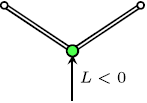
\includegraphics[scale= 0.7]{img_memory/entry.png}&  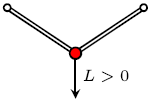
\includegraphics[scale= 0.7]{img_memory/exit.png}   & 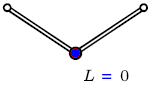
\includegraphics[scale= 0.7]{img_memory/junction.png} \\ \hline
    Control Mode &1. Pressure & 1. Outflow & \\
             & \footnotesize{\cred{\quad (Remi St)}}& \footnotesize{\cred{(Consumption)}} & \\
             &2. Inflow   &         & \\
             &\footnotesize{\cred{\quad  (Injection)}}&        & \\    \hline
    \end{tabular} 
    
    \caption{Classifications of \cnodes{non-pipe elements} attached to nodes.}
\end{table}

 %one is dividing by categories related to direction of the flux: exit, entrance or junction as is shown in Fig. \ref{tab: non_pipe_to_node_scheme_table}, pressure- or flux- regulated.   


%The taxonomy of the stations can be divided in different manners,


In Figure \ref{fig: schematic_remi},  an scheme of the operation of a REMI station its shown.

% Please add the following required packages to your document preamble:
% \usepackage{multirow}
\begin{table}[H]
\centering
\caption{Taxonomy of None pipe elements classified by type of constraints.}
\begin{tabular}{llll}
\hline
\multicolumn{2}{l}{Constraint type}             & Description        & Action at failure                             \\ \hline
\multirow{2}{*}{Hard} & Internal                & Intrinsic          & \multirow{2}{*}{Change} \\
                      & External & Operation limit    &                      \\ \hline
\multirow{2}{*}{Soft} & Internal                & Intrinsic          & \multirow{2}{*}{Warning/Change}               \\
                      & External & Working conditions & \\ \hline        
    \end{tabular}
    \label{tab: taxonomy station}
\end{table}

In Fig. an example of a remi station is given.

\begin{figure}[H]
    \centering
    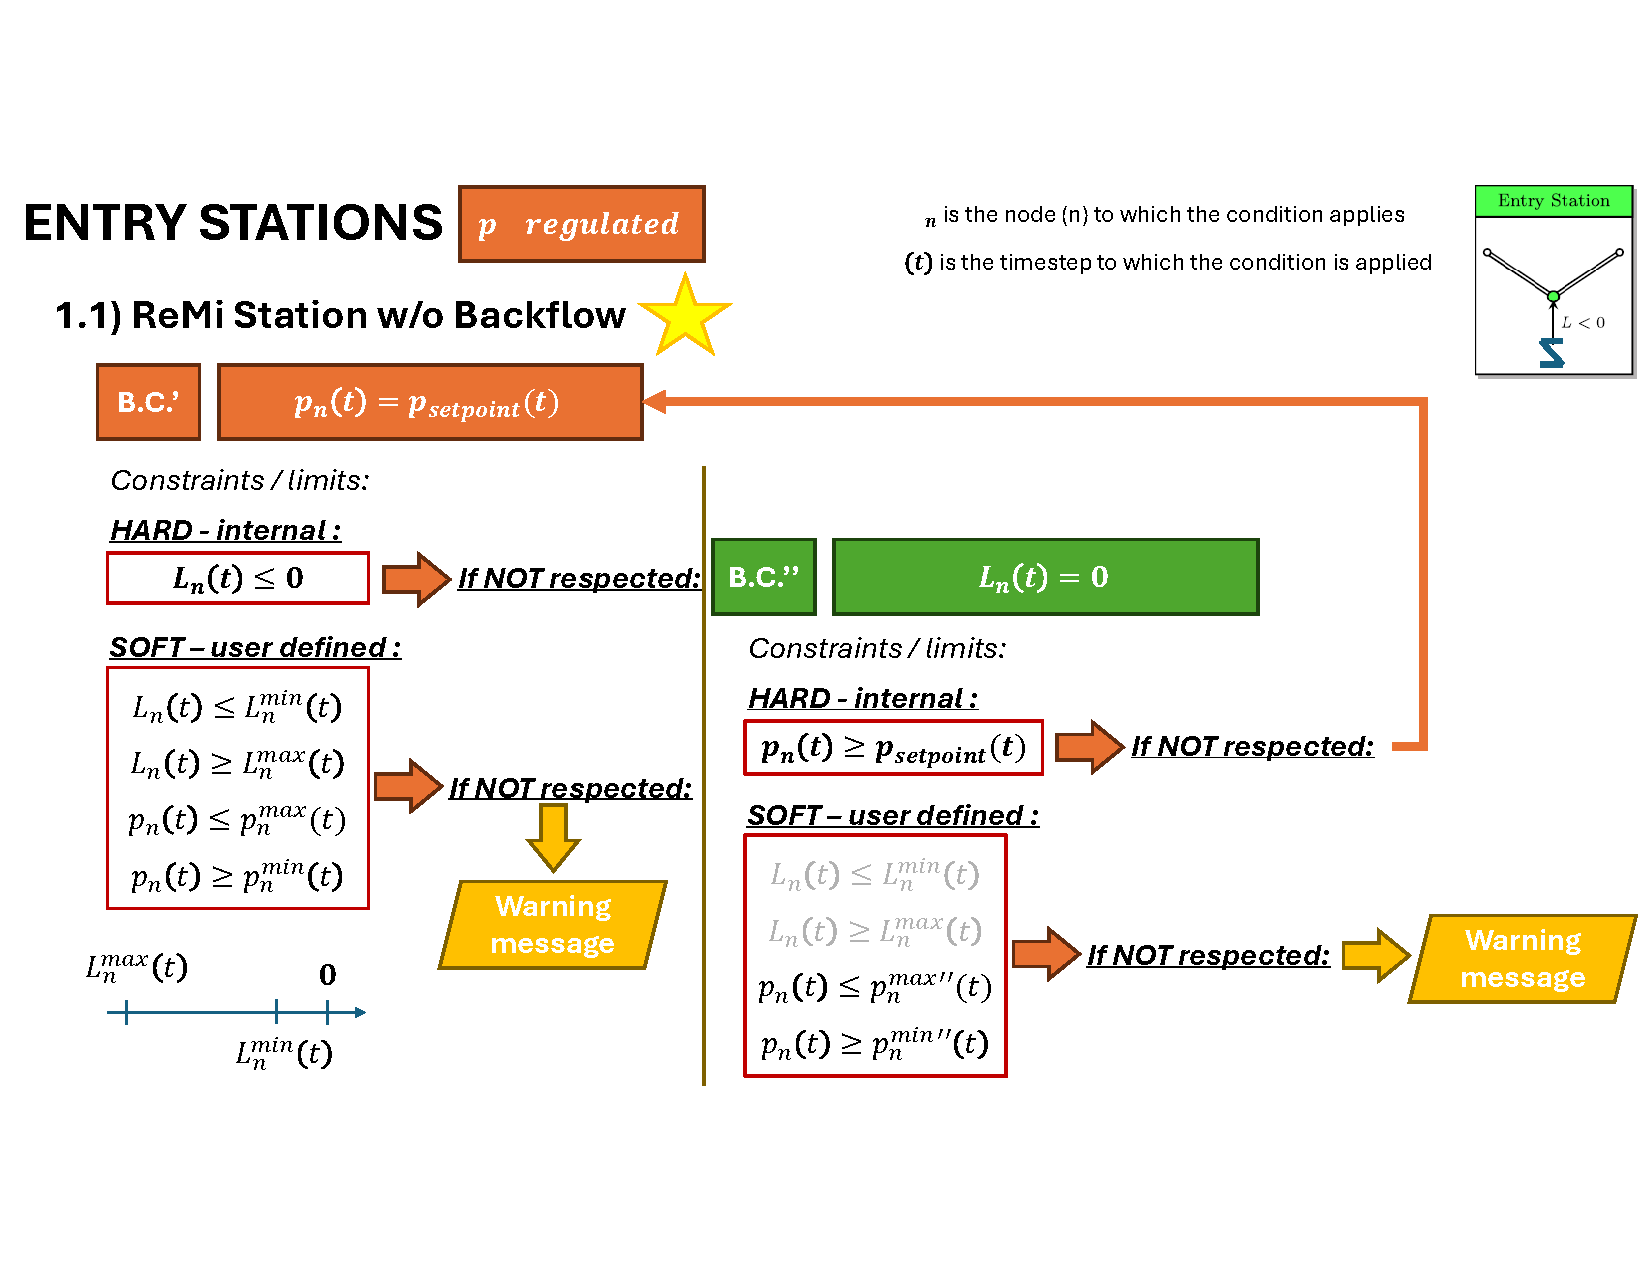
\includegraphics[scale=0.5]{img_memory/remi.pdf}
    \caption{Remi scheme. Courtesy of DENERG.}
    \label{fig: schematic_remi}
\end{figure}


\cstate{State}: 
\begin{itemize}
    \item Boundary
    \item Hard constraints
    \item Soft constraints
\end{itemize}


\cred{Remi w/o backflow}: entry station

    \begin{tabular}{|l|c|c|}
\hline
             & First \cstate{state}     &  Second \cstate{state} \\ \hline
    Boundary & $p = Pset$  & $L = 0$\\ 
    Hard constr.& $L \leq 0 $ & $p \geq Pset$\\ 
    Soft constr.& $L_{min}\leq L \leq  L_{max}$ & $L'_{min}\leq L \leq  L'_{max}$ \\
    & $p_{min}\leq p \leq  p_{max}$ & $p'_{min}\leq L \leq  p'_{max}$ \\\hline
    \end{tabular}


One can conclude that the main characteristic of the stations is that they are governed by states, which changes when hard constraints are violated. Each state encapsulates information about the boundary condition to be imposed, as well as the operational constraints and limits.
\begin{minted}[linenos=false,numbersep=1pt,frame=single,framesep=2mm,escapeinside=||]{cpp}
class |\textbf{\cred{station}}|
{
    std::vector<|\textbf{\cstate{state}}|> states_;

    void set_state(const |\textbf{\cstate{state}}|& s);   
};
\end{minted}

\begin{minted}[linenos=false,numbersep=1pt,frame=single,framesep=2mm,escapeinside=||]{cpp}
struct |\textbf{\cstate{state}}|
{
    |\textbf{\cblue{constraint}}|  boundary;  
    |\textbf{\cblue{constraint}}|  hards;
    std::vector<|\textbf{\cblue{constraint}}|> softs;
};
\end{minted}

\begin{minted}[linenos=false,numbersep=1pt,frame=single,framesep=2mm,escapeinside=||]{cpp}
class |\textbf{\cblue{constraint}}|
{
    hardness_type     hardness_;
    constraint_type   type_;
    vector_t          values_;
};
\end{minted}


In order to add a new kind of station, a function must be created in the file boundary.h using either an object of type \texttt{one\_state\_station} or \texttt{multiple\_states\_station}. 


\subsubsection{One state station}

For the sake of simplicity, let us add as an example the \texttt{consumption\_wo\_press}.  Since there are no switch states, this station is defined as a one state station object. Inside the function only a state is defined, which implies a boundary, a hard constraint and the soft constraints.
The function \texttt{build\_user\_constraints} defines the state components for each of the user-defined constraints, in an analogous manner to what was done for boundary and hard constraint types. The only difference is that \texttt{hardness\_type::SOFT} must be used and multiple constraints are allowed.
\begin{minted}[linenos=false,numbersep=1pt,frame=single,framesep=2mm,escapeinside=||]{cpp}
template<typename VALUE>
one_state_station
make_consumption_wo_press(const VALUE& vals,
                        const std::vector<pair_input_t>&user_limits)
{
    // Define the state components
    auto s0_bnd = constraint(hardness_type::BOUNDARY,  // Set as boundary 
                             constraint_type::L_EQUAL, // Only L_EQUAL or P_EQUAL 
                             vals);                    // Boundary condition values 

    auto s0_int = constraint(hardness_type::HARD,      // Set as hard constraints             
                             constraint_type::L_GREATER_EQUAL, // Inequalities 
                             0.0);                     // Limit of the inequality
    
    auto s0_ext = build_user_constraints(user_limits); // Create soft constraints

    // Create the state
    auto s0 = state(s0_bnd, s0_int, s0_ext);
    
    // Define the object consumption_station and give it a name
    one_state_station    consumption_station("CONSUMPTION_WO_PRESSURE"); 
    
    // Add the state to the station
    consumption_station.set_state(s0);

    return consumption_station;
}
    \end{minted}

\subsubsection{Multiple states station}  
        
For station with more than one state, you should use \texttt{multiple\_state\_station} class. 
You are able to define stations with more than 2 states also. Just use  the function {set\_state} to add as many states as you please. \\
    
For example a two sate station: 
\begin{minted}[linenos=false,numbersep=1pt,frame=single,framesep=2mm,escapeinside=||]{cpp}
    multiple_states_station remi("REMI_WO_BACKFLOW");
    remi.set_state(s0);
    remi.set_state(s1);
\end{minted}
In the case of an hypothetical 3 states station, the quantity of states must be provided.

\begin{minted}[linenos=false,numbersep=1pt,frame=single,framesep=2mm,escapeinside=||]{cpp}
    multiple_states_station    hypo("HYPOTHETICAL STATION", 3);
    hypo.set_state(s0);
    hypo.set_state(s1);        
    hypo.set_state(s2);              
\end{minted}    
The complete definition of the station is done as shown for the \texttt{one\_state\_station}            
                 
\begin{minted}[linenos=false,numbersep=1pt,frame=single,framesep=2mm,escapeinside=||]{cpp}
template<typename VALUE_TYPE>
multiple_states_station
make_remi_wo_backflow(  const VALUE_TYPE& Pset,
                         const std::vector<pair_input_t>& user_limits_s0,
                         const std::vector<pair_input_t>& user_limits_s1)
{
  using hard_t   = hardness_type;
  using constr_t = constraint_type;
  
   // 1. STATES
   // 1.1 Define the first state
  auto s0_bnd = constraint(hard_t::BOUNDARY, constr_t::P_EQUAL, Pset);
  auto s0_int = constraint(hard_t::HARD,     constr_t::L_LOWER_EQUAL, 0.0); 
  auto s0_ext = build_user_constraints(user_limits_s0);
 
  // 1.2 Define the second state
  auto s1_bnd = constraint(hard_t::BOUNDARY, constr_t::L_EQUAL, 0.0); 
  auto s1_int = constraint(hard_t::HARD,     constr_t::P_GREATER_EQUAL, Pset);
  auto s1_ext = build_user_constraints(user_limits_s1);

  // 1.3 Create states
  auto s0 = state(s0_bnd, s0_int, s0_ext);
  auto s1 = state(s1_bnd, s1_int, s1_ext);
 
  // 2. STATION
  // 2.1 Create station    
  multiple_states_station remi("REMI_WO_BACKFLOW");
  
  // 2.2 Add states
  remi.set_state(s0);
  remi.set_state(s1);

  return remi;
}
\end{minted}

